
% https://developers.facebook.com/
\subsubsection{Authentication} \label{sec:authencticationChallenge}

Authentication is an important aspect to our application. If the users are not authenticated correctly, one using the client cannot be sure that he is in fact communication with the one he expects. \smallskip

Authenticating yourself to another entity is impossible to do without either a third party or providing some evidence from real life that only the two of you can know. Since we do not want all of our clients to have to exchange something physical, we will go with the first approach of using a third party. \smallskip

Common practice for most mobile applications nowadays wanting authentication is to take advantage of Facebook. Facebook provides an API for developers, allowing their apps to be logged into from Facebook. This is the approach our application will take advantage of. An example of how the Facebook authentication looks can be seen in figure \figref{fig:FacebookAuthentication}.

\begin{figure}[H]
    \centering
    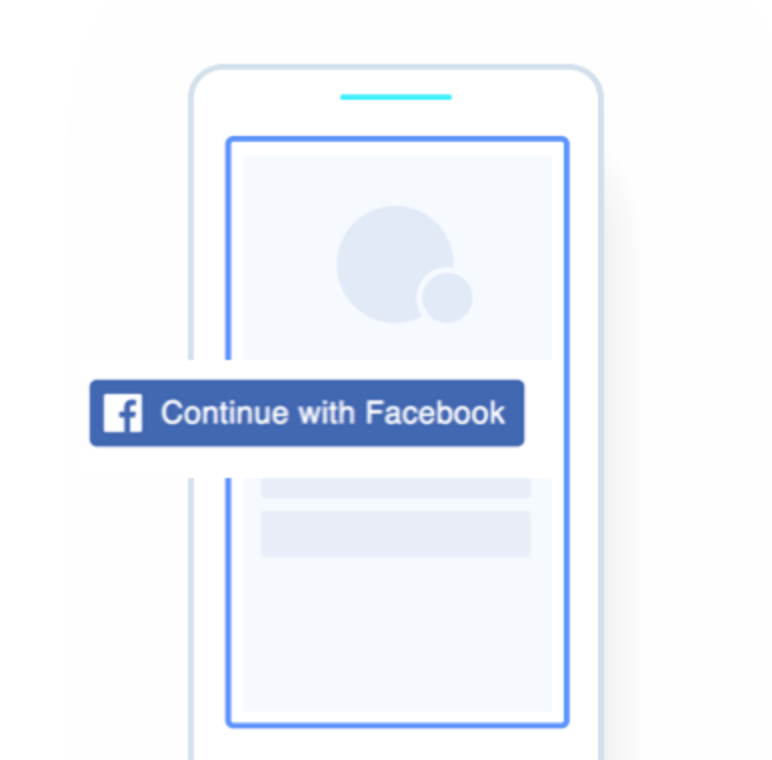
\includegraphics[width=0.65\textwidth]{images/FacebookLogin.png}
    \caption{Facebook authentication \cite{facebookApi}}
    \label{fig:FacebookAuthentication}
\end{figure}

It is noteworthy to mention that this solution does not actually authenticate a person, but rather authenticates them in regards to a Facebook profile. Thus if the Facebook profile is not actually sincere, neither will the user be on our platform. Other users interacting with this account will however know which Facebook profile it is connected to, so if a problem exists then its roots lies with Facebook authentication rather than ours.